% outline:
%%%%% Pronounciation
%%%%% What is LaTeX?
%%%%% Environment
%%%%% 

% \subsection{What is \LaTeX{}?}
\frame{
\frametitle{Pronunciation Guide}
    \begin{itemize}
        \item[\checkmark] Lah-tek
        \item[\checkmark] Lay-tek
        \item[$\times$] Lay-teks 
    \end{itemize}
}


\begin{frame}[fragile]
\frametitle{Where did \LaTeX{} come from?}
    \textbf{Donald Knuth} designed and wrote TeX in the late 1970s, during revisions of the second volume of his foundational work, \emph{The Art of Computer Programming}; created TeX in response to low-quality typography from publishers. \\ [\baselineskip]
    \emph{TeX} (= Tau Epsilon Chi) is a computer language designed for use in typesetting; in particular, for typesetting math and other technical material. \\[\baselineskip]
    Etymology: \textit{(from Greek ``techne" = art/craft, the stem of `technology') } \\[\baselineskip]
    {\scriptsize\itshape ``Science is knowledge which we understand so well that we can teach it to a computer; and if we don't fully understand something, it is an art to deal with it... In this sense, we should continually be striving to transform every art into a science: in the process, we advance the art." --- Donald Knuth, 1974 Turing Award Lecture}
\end{frame}


\begin{frame}[fragile]
\frametitle{Where did \LaTeX{} come from?}
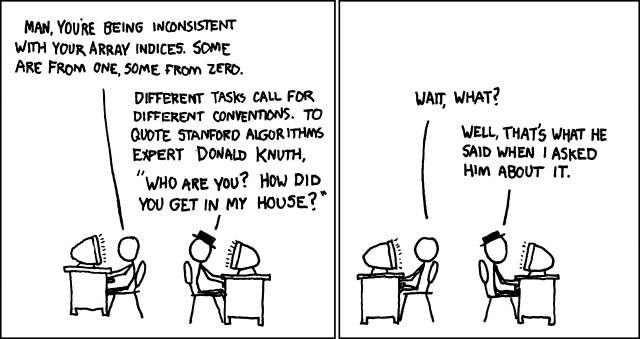
\includegraphics[width=\linewidth]{img/knuth_xkcd.png}
\hspace*{10pt}\hbox{\tiny Alt text: \thinspace{\tiny\itshape His books were kinda intimidating; rappelling down through his skylight seemed like the best option.}} \\
\hspace*{10pt}\hbox{\tiny Image credit:\thinspace{\tiny\itshape \url{https://xkcd.com/163}}} \\
\end{frame}


\frame{
\frametitle{What is \LaTeX{}?}
\LaTeX{} is ... \pause 
\begin{itemize}
    \item A macro package for the TeX programming language \pause
    \item A \textbf{typesetting program} for: \pause
    \begin{itemize}
        \item[$\bullet$] Mathematics \pause
        \item[$\bullet$] Non-Latin scripts (Arabic, Greek, etc.) \pause
    \end{itemize}
    \item Used as a scientific \textbf{document preparation system} for: \pause
    \begin{itemize}
        \item[$\bullet$] STEM Fields (mathematics, physics, computer science, engineering, chemistry, etc.) \pause 
        \item[$\bullet$] non-STEM Fields (economics, linguistics, psychology, philosophy, political science) \pause
    \end{itemize}
\end{itemize}
\begin{exampleblock}{}
    \LaTeX{} lives in between the worlds of \textbf{programming languages} (C, Java, Python, etc.) and \textbf{markup languages} (HTML, XML, etc.). 
\end{exampleblock}
}


\begin{frame}[fragile]
\frametitle{What's special about \LaTeX{}?}
    What separates \LaTeX{} from word processors like Microsoft Word or Google Docs? \pause
    \begin{itemize}
        \item[$\bullet$] \LaTeX{} follows the design principle of separating \emph{content} from \emph{presentation}. \pause
        \item[$\bullet$] The logical \emph{structure} of a document is handled by the author. \pause 
        \item[$\bullet$] Tools like \texttt{chapter, section, table, figure} and more are used to logically structure content without worrying about visual presentation. \pause
        \item[$\bullet$] Manual typesetting is possible, but the majority of adjustments are handled directly by \LaTeX{} itself. \pause
    \end{itemize}
    \vspace{0.1cm}
    \begin{center}
    \Large \LaTeX{} is a \emph{typesetting system}, not a word processor.
    \end{center}
\end{frame}

\begin{frame}[fragile]
\frametitle{Why use \LaTeX{}?}
    With \LaTeX{}, you can... \pause
    \begin{itemize}
        \item[$\bullet$] Create professional looking documents. \pause
        \item[$\bullet$] Create complex documents \emph{fast}. \pause
        \item[$\bullet$] Easily include beautiful mathematical expressions, figures, etc. in a document. \pause
        \item[$\bullet$] Edit images directly at any time. \pause
        \item[$\bullet$] Create dynamic internal references easily. \pause
        \item[$\bullet$] Maintain consistent formatting throughout documents. \pause
        \item[$\bullet$] Focus on content (no more stress about manual formatting!).
    \end{itemize}
\end{frame}

\begin{frame}[fragile]
\frametitle{Why use \LaTeX{}?}
    Learning \LaTeX{} is a little bit like... \\ \pause
    \vspace{0.1cm}
    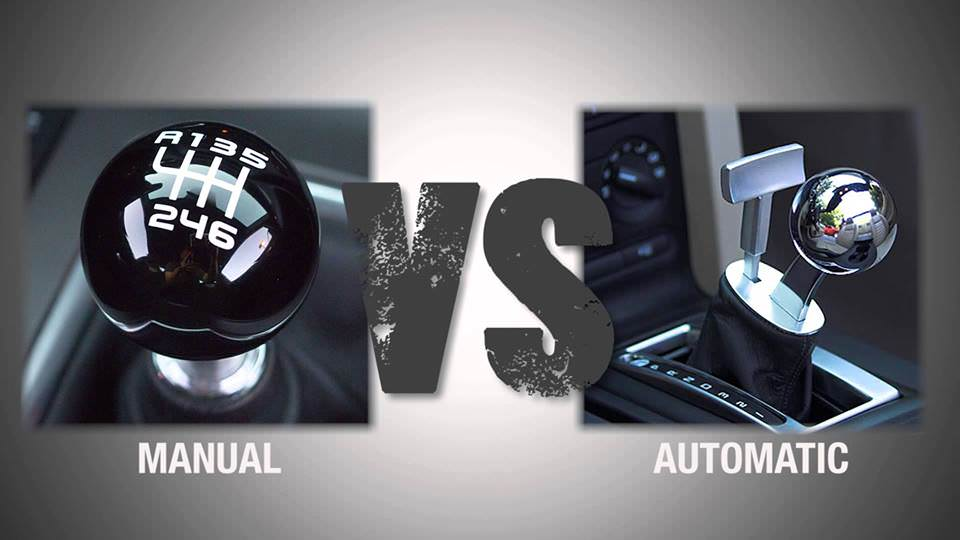
\includegraphics[width=\linewidth]{img/man_auto.jpg}
    \hspace*{15pt}\hbox{\tiny Image credit:\thinspace{\tiny\itshape AIS Insurance Specialists Blog}}
\end{frame}


\begin{frame}[fragile]
\frametitle{Should YOU be using \LaTeX{}?}
    \begin{columns}
    \small
    \column{0.5\linewidth}
        \textbf{You \emph{should} use \LaTeX{} if...} \pause
        \begin{itemize}
            \item[$\bullet$] You work in academia or research. \pause
            \item[$\bullet$] You write documents with lots of equations. \pause
            \item[$\bullet$] You work with long bibliographies. \pause
            \item[$\bullet$] You want to forget about document layout. \pause
            \item[$\bullet$] You want quality {\footnotesize(SVG)} figures. \pause
            \item[$\bullet$] You want forward-compatibility \pause
            \item[$\bullet$] You want your documents to stand out. \pause
        \end{itemize}
    \column{0.5\linewidth}
        \textbf{You should \emph{not} use \LaTeX{} if...} \pause
        \begin{itemize}
            \item[$\bullet$] You don't have time (or the patience) to learn how to use it. \pause
            \item[$\bullet$] You want real-time collaboration with non-\LaTeX{} people. \pause
            \item[$\bullet$] You want to manually control/edit every graphical aspect of a document. \pause
            \item[$\bullet$] You need to exchange working documents with non-\LaTeX{} people. \pause
            \item[$\bullet$] You prefer ``quick and easy." 
        \end{itemize}
    \end{columns}
\end{frame}


\begin{frame}[fragile]
\frametitle{What's \emph{This} Course For?}
    \begin{itemize}[$\bullet$]
        \item Overview of the \LaTeX{} typesetting language.
        \item Demonstrate how to create professional \textit{looking} documents. 
        \item Provide bite-size problems to solve.
    \end{itemize}
\end{frame}




% \subsection{\LaTeX{} Environments}

\begin{frame}
\frametitle{\LaTeX{} Software Packages}
\begin{columns}
\column{0.5\textwidth}
\begin{center}

\includegraphics[width=0.75\textwidth]{img/texlive_logo.png}
{\small \url{https://www.tug.org/texlive/}}

\includegraphics[width=0.5\textwidth]{img/texworks_logo.jpg}
{\small \url{https://tug.org/texworks/}}
\end{center}

\column{0.5\textwidth}
\begin{center}

\includegraphics[width=0.5\textwidth]{img/mactex_logo.png} \\
{\small \url{https://www.tug.org/mactex/}}

\includegraphics[width=0.5\textwidth]{img/texshop_logo.jpg} \\
{\small \url{https://pages.uoregon.edu/koch/texshop/}}
\end{center}
\end{columns}
\end{frame}


\frame{
\frametitle{Cloud-Based \LaTeX{} Editor}
\begin{center}

\includegraphics[width=0.6\linewidth]{img/overleaf_logo.png} \\ 
\url{https://www.overleaf.com} \\
\vspace{1cm}
\begin{exampleblock}{Advantages}
    Many templates, commonly used, collaborative, well-documented and free!
\end{exampleblock}
\end{center}
}


\frame{
\frametitle{Window Layout}
\begin{columns}
\column{0.2\textwidth}
\begin{center}
Files
\end{center}

\column{0.3\textwidth}
\begin{center}
Editor
\end{center}

\column{0.4\textwidth}
\begin{center}
Output Document
\end{center}
\end{columns}

\begin{center}
    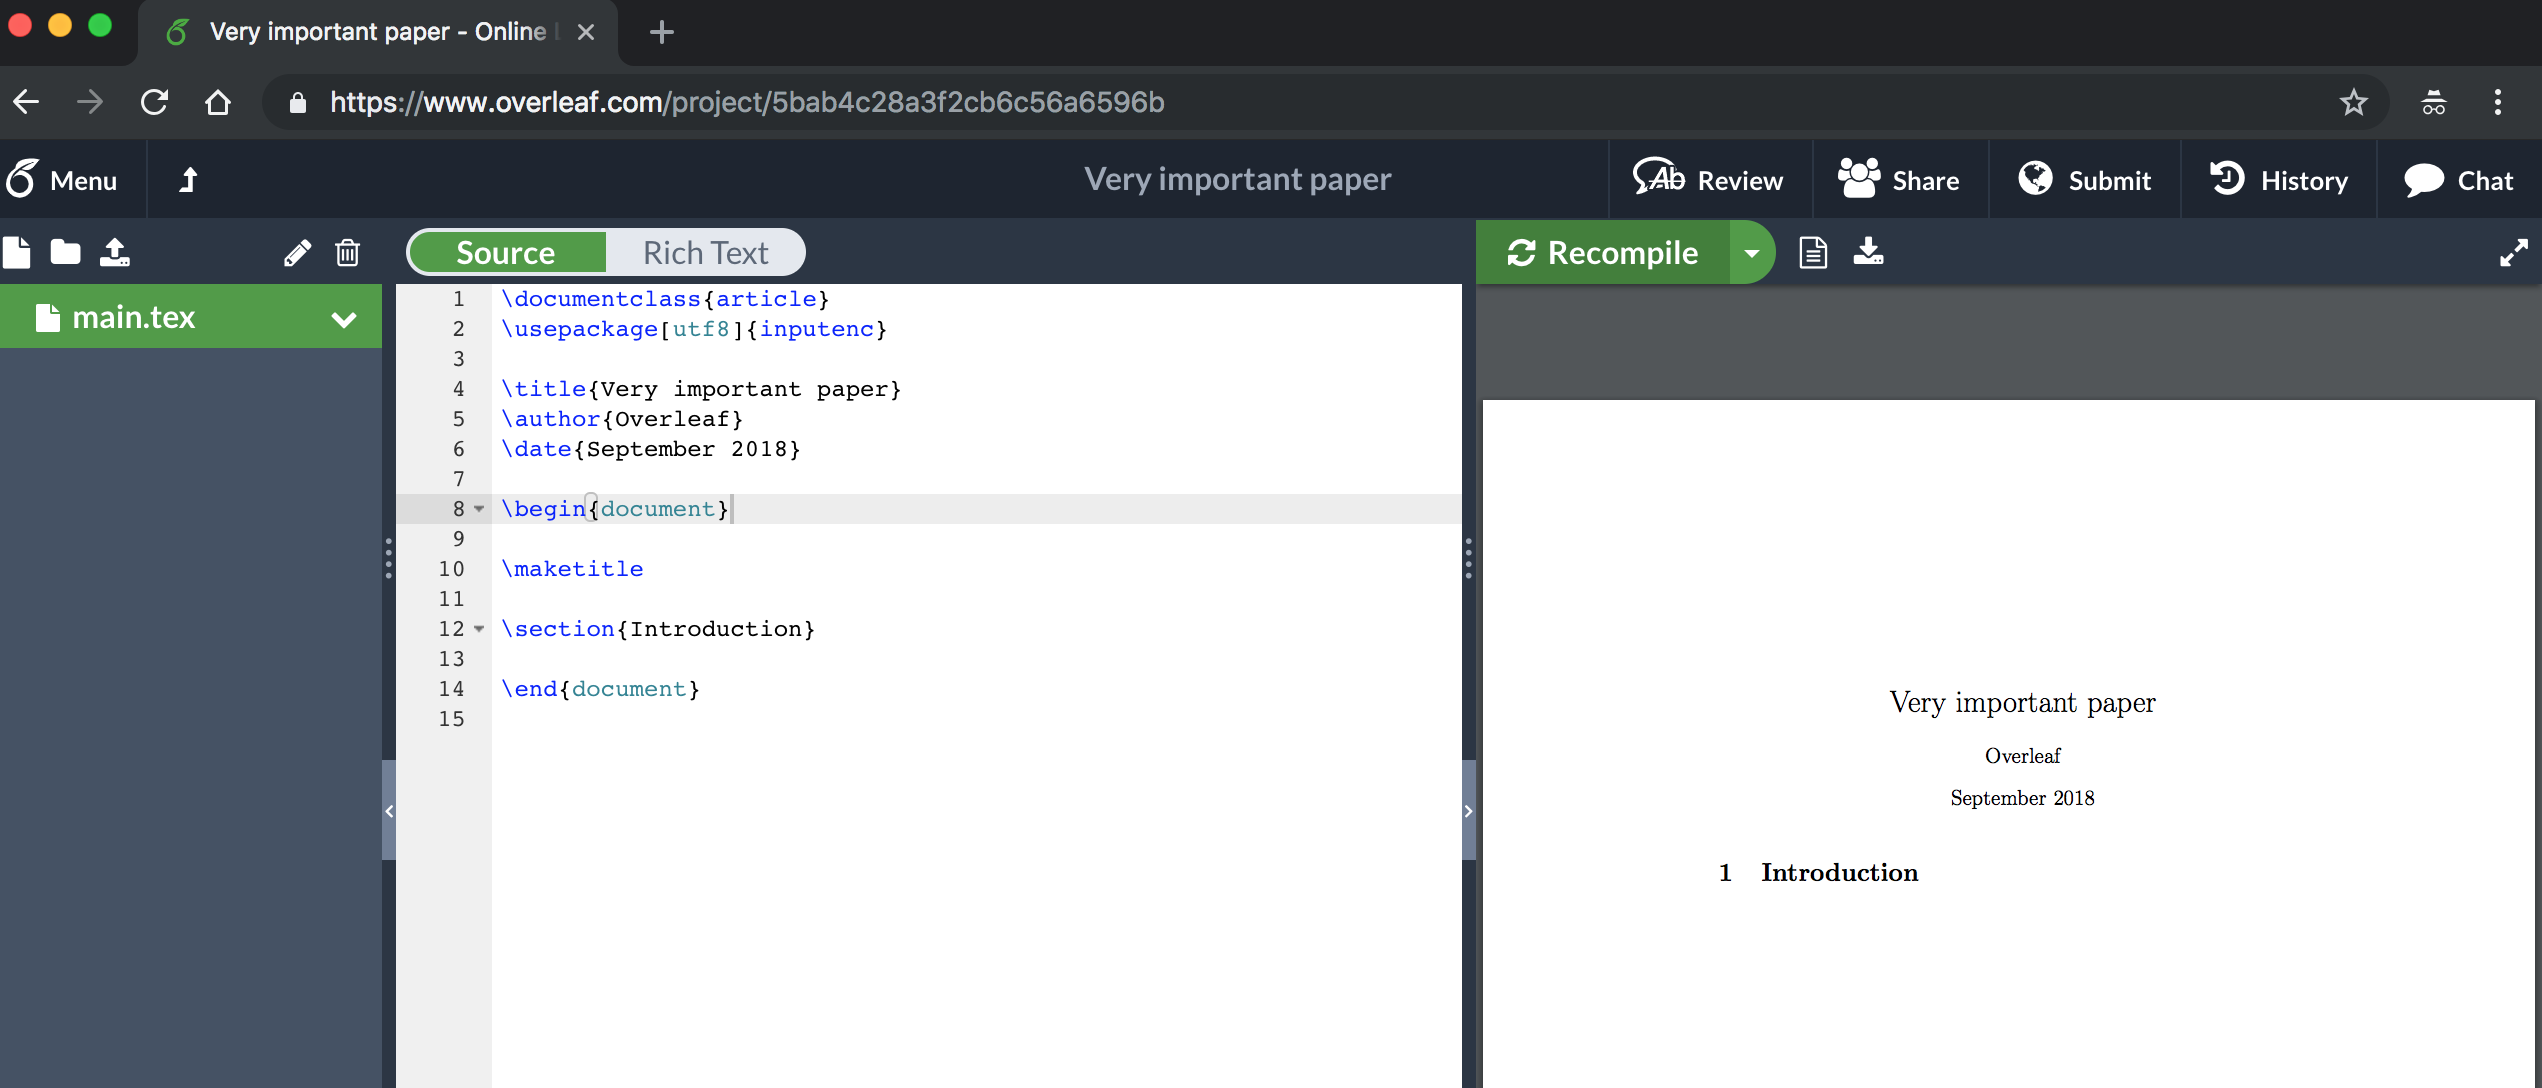
\includegraphics[width=\textwidth]{img/overleaf_windows.png}
\end{center}
}

% {\setbeamercolor{background canvas}{bg=red!15}
% \begin{frame}{This frame is red}
% \end{frame}
% }

% 
% {\setbeamercolor{background canvas}{bg=red!15}
\begin{frame}[fragile]
\frametitle{Exercise: Getting Started \\
{\small Examples and exercises are developed and shown in Overleaf.}} 
\begin{itemize}
    \item[$\bullet$] Open your \LaTeX{} editor of choice.
    \item[$\bullet$] New Project~\rightarrow~Blank Project \rightarrow~\textit{(Title)} 
    \item {\small \textit{This will open a blank project containing the file \texttt{main.tex}.}} 
    \item[$\bullet$] Delete (or comment out) any text and/or commands automatically included in the file.
    \item {\small \textit{We're going to rewrite most of it step-by-step.}} 
\end{itemize}
\begin{alertblock}{}
    \begin{minted}{latex}
    % percentage symbol indicates the start of a  
    % comment.
    % this is a great way to take notes directly 
    % in your document.
    \end{minted}
\end{alertblock}

\end{frame}
% }



\begin{frame}[fragile]
\frametitle{Before we begin:}
\begin{itemize}
    \item[$\bullet$] To comment: \keytt{\% comment text}
    \item Or for longer comments, load \verb|\usepackage{comment}| and use commands \verb|\begin{comment} ... \end{comment}|
    \item[$\bullet$] Compile frequently!
    \item Ctrl + S
    \item Recompile button
    \item For faster compilation, use \textit{Fast (draft) compile mode}.
    \item Recommended to compile from main document.
\end{itemize}
\end{frame}

